\documentclass[a4paper]{article}

\usepackage{amsmath}
\usepackage{booktabs}
\usepackage{numprint}

% Per i plot
\usepackage{pgfplots}
\usepackage{pgf-pie} 

\usepackage{tabstackengine,xcolor,rotating}
\newcommand\blackcard[2]{%
    \begingroup\fboxsep=0pt\relax
    \fbox{\tabbedCenterstack{%
    \hspace{3pt}\scriptsize$#2$ && \\ &\makebox[10pt]{#1}& \\ &&\rotatebox[origin=c]{180}{\scriptsize$#2$}\hspace{3pt}}}%
    \endgroup}
\newcommand\redcard[2]{%
    \begingroup\fboxsep=0pt\relax
    \fbox{\color{red}\tabbedCenterstack{%
    \hspace{3pt}\scriptsize$#2$ && \\ &\makebox[10pt]{#1}& \\ &&\rotatebox[origin=c]{180}{\scriptsize$#2$}\hspace{3pt}}}%
    \endgroup}
\newcommand\bluecard[2]{%
    \begingroup\fboxsep=0pt\relax
    \fbox{\color{blue}\tabbedCenterstack{%
    \hspace{3pt}\scriptsize$#2$ && \\ &\makebox[10pt]{#1}& \\ &&\rotatebox[origin=c]{180}{\scriptsize$#2$}\hspace{3pt}}}%
    \endgroup}

\usepackage{listings}

\definecolor{codegray}{rgb}{0.5,0.5,0.5}
\definecolor{codepurple}{rgb}{0.58,0,0.82}
\definecolor{backcolour}{rgb}{0.95,0.95,0.92}
\lstdefinestyle{mystyle}{
    backgroundcolor=\color{backcolour},
    keywordstyle=\color{blue},
    numberstyle=\tiny\color{codegray},
    stringstyle=\color{codepurple},
    basicstyle=\ttfamily\footnotesize,
    numbers=left,
    breaklines=true,
    numbersep=-10pt,
    tabsize=2
}
\lstset{style=mystyle}

\begin{document}

\begin{titlepage}
    \title{Solitario di Prina}
    \author{Gallina Roberto}
    \date{13/11/2022}
    \maketitle
\end{titlepage}

\newpage

\tableofcontents

\newpage

\section{Premesse}
In tutto il documento ci si riferirà a il \emph{mazzo (Deck)}, esso è da intendere come un mazzo di 40 carte, divise in 4 semi. Per convenzione durante il documento si userà il mazzo francese le cui carte sono:

\begin{itemize}
    \item l'asso
    \item il due
    \item il tre
    \item il quattro
    \item il cinque
    \item il sei
    \item il sette
    \item il fante (J)
    \item la regina (Q)
    \item il re (K)
\end{itemize}

\noindent
Mentre i semi sono:

\begin{itemize}
    \item i cuori
    \item i quadri
    \item i fiori
    \item i picche
\end{itemize}

\noindent
Il mazzo è quindi composta dalle carte sottostanti:
\begin{figure}[h]
    \centering
    \scalebox{0.8}{
        \redcard{1}{\heartsuit}
        \redcard{2}{\heartsuit}
        \redcard{3}{\heartsuit}
        \redcard{4}{\heartsuit}
        \redcard{5}{\heartsuit}
        \redcard{6}{\heartsuit}
        \redcard{7}{\heartsuit}
        \redcard{J}{\heartsuit}
        \redcard{Q}{\heartsuit}
        \redcard{K}{\heartsuit}
    }
    \scalebox{0.8}{
        \redcard{1}{\diamondsuit}
        \redcard{2}{\diamondsuit}
        \redcard{3}{\diamondsuit}
        \redcard{4}{\diamondsuit}
        \redcard{5}{\diamondsuit}
        \redcard{6}{\diamondsuit}
        \redcard{7}{\diamondsuit}
        \redcard{J}{\diamondsuit}
        \redcard{Q}{\diamondsuit}
        \redcard{K}{\diamondsuit}
    }
    \scalebox{0.8}{
        \blackcard{1}{\clubsuit}
        \blackcard{2}{\clubsuit}
        \blackcard{3}{\clubsuit}
        \blackcard{4}{\clubsuit}
        \blackcard{5}{\clubsuit}
        \blackcard{6}{\clubsuit}
        \blackcard{7}{\clubsuit}
        \blackcard{J}{\clubsuit}
        \blackcard{Q}{\clubsuit}
        \blackcard{K}{\clubsuit}
    }
    \scalebox{0.8}{
        \blackcard{1}{\spadesuit}
        \blackcard{2}{\spadesuit}
        \blackcard{3}{\spadesuit}
        \blackcard{4}{\spadesuit}
        \blackcard{5}{\spadesuit}
        \blackcard{6}{\spadesuit}
        \blackcard{7}{\spadesuit}
        \blackcard{J}{\spadesuit}
        \blackcard{Q}{\spadesuit}
        \blackcard{K}{\spadesuit}
    }
    \caption{Mazzo}
\end{figure}

In tutto il documento ci si riferirà a la \emph{sequenza}, essa rappresenta l'ordine delle carte nel mazzo mescolato.

\newpage

\section{Funzionamento del gioco}

Il gioco è molto semplice, dato un mazzo da gioco mischiato, si tengono tutte le carte coperte in pila; si scopre le prime tre carte.
Nel caso la prima e la terza carta hanno stesso valore o stesso seme, allora la seconda carta viene spostasta sopra la prima (avvicinando la terza).
Successivamente si scopre un'altra carta di ricomincia a controllare dall'inizio.

\vspace{0.5cm}
Ecco un esempio del funzionamento
\begin{figure}[h]
    \centering
    \scalebox{0.8}{
        \blackcard{1}{\spadesuit}
    }
    \\
    \vspace{0.5cm}
    \scalebox{0.8}{
        \blackcard{1}{\spadesuit}
        \redcard{K}{\diamondsuit}
    }
    \\
    \vspace{0.5cm}
    \scalebox{0.8}{
        \blackcard{1}{\spadesuit}
        \redcard{K}{\diamondsuit}
        \blackcard{1}{\clubsuit}
    }\\
    \vspace{0.5cm}
    \scalebox{0.8}{
        \bluecard{1}{\spadesuit}
        \redcard{K}{\diamondsuit}
        \bluecard{1}{\clubsuit}
    }
    \\
    \vspace{0.2cm}
    Avendo lo stesso valore (1), la carte centrale sale sopra la prima
    \\
    \vspace{0.5cm}
    \scalebox{0.8}{
        \redcard{K}{\diamondsuit}
        \blackcard{1}{\clubsuit}
    }
    \caption{Esempio di funzionamento}
\end{figure}

\newpage

\subsection{Sequenza corretta}

Viene definita \emph{sequenza corretta}, una sequenza, in cui terminate le carte si hanno due esattamente due pile di carte.

\vspace{0.5cm}
Eccone un esempio
\begin{figure}[h]
    \centering
    \scalebox{0.8}{
        \blackcard{4}{\spadesuit}
        \redcard{5}{\heartsuit}
        \blackcard{4}{\clubsuit}
        \redcard{3}{\heartsuit}
        \redcard{K}{\heartsuit}
        \redcard{2}{\heartsuit}
        \blackcard{K}{\clubsuit}
        \redcard{K}{\diamondsuit}
        \blackcard{7}{\spadesuit}
        \blackcard{1}{\spadesuit}
    }
    \scalebox{0.8}{
        \redcard{6}{\heartsuit}
        \blackcard{3}{\clubsuit}
        \redcard{Q}{\heartsuit}
        \redcard{1}{\diamondsuit}
        \blackcard{2}{\clubsuit}
        \blackcard{Q}{\clubsuit}
        \redcard{7}{\heartsuit}
        \blackcard{3}{\spadesuit}
        \blackcard{5}{\clubsuit}
        \redcard{7}{\diamondsuit}
    }
    \scalebox{0.8}{
        \blackcard{Q}{\spadesuit}
        \redcard{5}{\diamondsuit}
        \redcard{1}{\heartsuit}
        \redcard{3}{\diamondsuit}
        \redcard{J}{\heartsuit}
        \redcard{Q}{\diamondsuit}
        \redcard{J}{\diamondsuit}
        \blackcard{J}{\spadesuit}
        \blackcard{2}{\spadesuit}
        \blackcard{1}{\clubsuit}
    }
    \scalebox{0.8}{
        \blackcard{7}{\clubsuit}
        \redcard{4}{\heartsuit}
        \blackcard{K}{\spadesuit}
        \redcard{4}{\diamondsuit}
        \blackcard{J}{\clubsuit}
        \redcard{6}{\diamondsuit}
        \blackcard{5}{\spadesuit}
        \blackcard{6}{\clubsuit}
        \redcard{2}{\diamondsuit}
        \blackcard{6}{\spadesuit}
    }
    \caption{Sequenza corretta}
\end{figure}

\subsection{Sequenza perfetta}

Viene definita \emph{sequenza perfetta}, una sequenza corretta, in cui è esattamente l'ultima carta a formare la seconda pila; per cui terminate le carte di hanno esattamente due pile di carte in cui la seconda pila ha esattamente una carta

\vspace{0.5cm}
Eccone un esempio
\begin{figure}[h]
    \centering
    \scalebox{0.8}{
        \redcard{1}{\heartsuit}
        \redcard{1}{\diamondsuit}
        \redcard{2}{\heartsuit}
        \redcard{2}{\diamondsuit}
        \redcard{3}{\heartsuit}
        \redcard{3}{\diamondsuit}
        \redcard{4}{\heartsuit}
        \redcard{4}{\diamondsuit}
        \redcard{5}{\heartsuit}
        \redcard{5}{\diamondsuit}
    }
    \scalebox{0.8}{
        \redcard{6}{\diamondsuit}
        \redcard{6}{\heartsuit}
        \redcard{7}{\diamondsuit}
        \redcard{7}{\heartsuit}
        \redcard{J}{\diamondsuit}
        \redcard{Q}{\heartsuit}
        \redcard{J}{\heartsuit}
        \redcard{Q}{\diamondsuit}
        \redcard{K}{\heartsuit}
        \redcard{K}{\diamondsuit}
    }
    \scalebox{0.8}{
        \blackcard{K}{\spadesuit}
        \blackcard{K}{\clubsuit}
        \blackcard{Q}{\spadesuit}
        \blackcard{Q}{\clubsuit}
        \blackcard{J}{\spadesuit}
        \blackcard{J}{\clubsuit}
        \blackcard{7}{\spadesuit}
        \blackcard{7}{\clubsuit}
        \blackcard{6}{\spadesuit}
        \blackcard{6}{\clubsuit}
    }
    \scalebox{0.8}{
        \blackcard{5}{\spadesuit}
        \blackcard{5}{\clubsuit}
        \blackcard{4}{\spadesuit}
        \blackcard{4}{\clubsuit}
        \blackcard{3}{\spadesuit}
        \blackcard{3}{\clubsuit}
        \blackcard{2}{\spadesuit}
        \blackcard{2}{\clubsuit}
        \blackcard{1}{\spadesuit}
        \blackcard{1}{\clubsuit}
    }
    \caption{Sequenza perfetta}
\end{figure}

\newpage

\subsection{Sequenza n-perfect}

Viene definita \emph{sequenza n-perfect}, una sequenza, in cui terminate le carte non ci sono pile con più di un carta, ossia il numero delle pile è uguale al numero delle carte

\vspace{0.5cm}
Eccone un esempio
\begin{figure}[h]
    \centering
    \scalebox{0.8}{
        \redcard{1}{\heartsuit}
        \redcard{1}{\diamondsuit}
        \blackcard{2}{\clubsuit}
        \blackcard{2}{\spadesuit}
        \redcard{3}{\heartsuit}
        \redcard{3}{\diamondsuit}
        \blackcard{4}{\clubsuit}
        \blackcard{4}{\spadesuit}
        \redcard{5}{\heartsuit}
        \redcard{5}{\diamondsuit}
    }
    \scalebox{0.8}{
        \blackcard{6}{\clubsuit}
        \blackcard{6}{\spadesuit}
        \redcard{7}{\heartsuit}
        \redcard{7}{\diamondsuit}
        \blackcard{J}{\clubsuit}
        \blackcard{J}{\spadesuit}
        \redcard{Q}{\heartsuit}
        \redcard{Q}{\diamondsuit}
        \blackcard{K}{\clubsuit}
        \blackcard{K}{\spadesuit}
    }
    \scalebox{0.8}{
        \redcard{2}{\heartsuit}
        \redcard{2}{\diamondsuit}
        \blackcard{1}{\clubsuit}
        \blackcard{1}{\spadesuit}
        \redcard{4}{\heartsuit}
        \redcard{4}{\diamondsuit}
        \blackcard{3}{\clubsuit}
        \blackcard{3}{\spadesuit}
        \redcard{6}{\heartsuit}
        \redcard{6}{\diamondsuit}
    }
    \scalebox{0.8}{
        \blackcard{5}{\clubsuit}
        \blackcard{5}{\spadesuit}
        \redcard{J}{\heartsuit}
        \redcard{J}{\diamondsuit}
        \blackcard{7}{\clubsuit}
        \blackcard{7}{\spadesuit}
        \redcard{K}{\heartsuit}
        \redcard{K}{\diamondsuit}
        \blackcard{Q}{\clubsuit}
        \blackcard{Q}{\spadesuit}
    }
    \caption{Esempio di sequeza n-perfect}
\end{figure}

\newpage

\section{Introduzione}
Durante le innumerevoli partite giocate da me giocate, non è capito che la sequenza fosse corretta o ben che meno perfetta, e quindi nata in me l'idea si sapere quanto siano rare tali sequenze, ho quindi iniziato ad analizzare il gioco dal punto di vista statistico.

Poichè il mazzo è composto da 40 carte, possiamo calcolare il numero totale di sequenze, esso sarà pari a $40! \simeq 8.1591528 \cdot 10^{47}$; questo numero computazionalmente enorme, non è quindi possibile su un computer verificare tutte le sequenze possibili per avere dati esatti.
Allo stesso modo anche calcolare quante siano le sequenze corrette, perfette o n-perfect non è semplice, avendo dati esempi di tutte e tre possiamo sicuramente affermare che ne esistano.

\section{Analisi statistica}

Definiamo $P_C$ la probabilità che una sequenza sia corretta, $P_P$ la probabilità che una sequenza sia perfetta e $P_{N-P}$ la probabilità che una sequenza sia n-perfect; queste probabilità sono a noi sconusciute, ma sicuramente $P_C>0$,  $P_P>0$ e $P_{N-P}>0$ avendo dato un esempio per ognuna.

Ci aspettiamo che su 10 sequenze, le sequenze corrette $S_{C}^{10}$ siano:
\begin{equation*}
    S_{C}^{10} \simeq 10 \cdot P_C
\end{equation*}

Possiamo quindi isolare $P_C$
\begin{equation*}
    P_C \simeq \frac{S_{C}^{10}}{10}
\end{equation*}

Ovviamente questa è un'approsimazione, ma aumentando il numero di sequenze otterremo un risultato sempre più vicino a $P_C$, possiamo quindi definire:
\begin{equation*}
    P_C =  \lim_{n \to +\infty} {\frac{S_{C}^{n}}{n}}
\end{equation*}

Allo stesso modo definiamo:
\begin{equation*}
    P_P =  \lim_{n \to +\infty} {\frac{S_{P}^{n}}{n}}
    \qquad
    \qquad
    P_{N-P} =  \lim_{n \to +\infty} {\frac{S_{N-P}^{n}}{n}}
\end{equation*}

Possiamo quindi scrivere un programma per generare quante più sequenze possibili in modo approssimare queste probabilità.

\newpage

\section{Implementazione}
Iniziamo col definire gli enumeratori per i semi e per i valori, in modo da poterli usare con semplicità dopo.

\begin{lstlisting}[language=Java]
    class Seme {
        public static HEART = "1";
        public static DIAMOND = "2";
        public static FLOWER = "3";
        public static CLUB = "4";
    }
\end{lstlisting}

\begin{lstlisting}[language=Java]
    class Value {
        public static ONE = "1";
        public static TWO = "2";
        public static THREE = "3";
        public static FOUR = "4";
        public static FIVE = "5";
        public static SIX = "6";
        public static SEVEN = "7";
        public static JACK = "J";
        public static QUEEN = "Q";
        public static KING = "K";
    }
\end{lstlisting}

\vspace{0.5cm}
\noindent
Definiamo ora una carta come una classe che memorizza un seme e un valore.

\begin{lstlisting}[language=Java]
    class Card{
        private Seme seme;
        private Value value;

        constructor(seme, value) {
            this.seme = seme;
            this.value = value;
        }

        public Seme getSeme() {
            return this.seme
        }

        public Value getValue() {
            return this.value
        }
    }
\end{lstlisting}

\vspace{0.5cm}
\noindent
Definiamo poi il mazzo come un contenitore di 40 carte; definiamogli poi:
\begin{itemize}
    \item un metodo $shuffle$ che randomicamente mischia le carte nel mazzo.
    \item un metodo $sameValueOrSeme$ che confronta due carte, ritornando $true$ se hanno lo stesso valore o lo stesso seme
    \item un metodo $check$ che data una sequenza di carte le confronta facendo salire quelle con lo stesso valore o seme, ritornando la sequenza ridotta
    \item un metodo $isCorrect$ che analizza la sequenza è dice se la sequenza ridotta è di 2 carte
    \item un metodo $isPerfect$ che analizza la sequenza è dice se la sequenza ridotta è di 2 carte (in cui l'ultima è esattamente l'ultima scesa)
    \item un metodo $isNPerfect$ che analizza la sequenza è dice se la sequenza ridotta è di 40 carte
\end{itemize}

La classe risultante sarà simile a questa
\begin{lstlisting}[language=Java]
    class Deck{
        private Card cards[40];

        constructor() {
            this.cards.add(new Card(Seme.HEART, Value.ONE));
            this.cards.add(new Card(Seme.DIAMOND, Value.ONE));
            .
            .
        }

        public void shaffle() { 
            cards.randomSort(); 
        }

        public bool sameValueOrSeme(a, b) {
            return a.value == b.value || a.seme == b.seme;
        }
    
        public Card[] check(cards) {
            i = 0;
            j = 2;
    
            while (j < cards.length) {
                if (sameValueOrSeme(cards[i], cards[j])) {
                    cards.removeByIndex(i);
                    i = 0;
                    j = 2;
                } else {
                    i++;
                    j++;
                }
            }
            return cards;
        }
    
        public bool isCorrect() {
            return check(cards).length == 2;
        }
    
        public bool isPerfect() {
            last = cards.pop();
            cards = check(cards);

            if (cards.length == 2) {
                return sameValueOrSeme(cards[0], last);
            }
            return false;
        }
    
        public bool isNPerfect() {
            return check(cards).length == 40;
        }
    }
\end{lstlisting}

\newpage

\noindent
Possiamo quindi scrivere un programma per calcolare sequenze corrette, perfette o n-perfect.

\begin{lstlisting}[language=Java]
    do {
        d = new Deck();
        d.shaffle();
    } while (d.isCorrect());
    // or d.isPerfect() or d.isNPerfect()

    d.print();  // is a method for print the sequence
\end{lstlisting}

\vspace{0.5cm}
\noindent
Oppure, ben più interessante, possiamo generare diverse sequenze contare quante di esse siano corrette, prefette o n-perfect

\begin{lstlisting}[language=Java]
    const MAX_TENT = 1 * 1000 * 1000;
    correct = 0;
    perfect = 0;
    n_perfect = 0;
    
    for (i = 0; i < MAX_TENT; i++) {
        d = new Deck();
        d.shaffle();
    
        if (d.isCorrect()) {
            correct++;
            if (d.isPerfect()) 
                perfect++
        }
        if (d.isNPerfect())
            n_perfect++;
    }
\end{lstlisting}

\vspace{0.5cm}
\noindent
Possiamo ora lanciare il programma generando \numprint{10}, \numprint{100}, \numprint{1000}, \numprint{10000}, \numprint{1000000}, \numprint{10 000 000}, \numprint{100 000 000} e \numprint{1 000 000 000} sequenze; vediamo il risultato

\begin{table}[htp]
    \centering
    \begin{tabular}{@{} c c c c c c c @{}}
        \toprule
        Sequenze & Sequenze & $P_C$      & Sequenze & $P_P$      & Sequenze  & $P_{NP}$   \\
        generate & corrette &            & perfette &            & n-perfect &            \\
        \midrule
        10       & 1        & $0.1$      & 0        & $0$        & 0         & $0$        \\
        $10^2$   & 2        & $2$        & 0        & $0$        & 0         & $0$        \\
        $10^3$   & 5        & $0.5$      & 1        & $0.1$      & 0         & $0$        \\
        $10^4$   & 42       & $0.42$     & 6        & $0.6$      & 0         & $0$        \\
        $10^5$   & 456      & $0.4559$   & 141      & $0.141$    & 0         & $0$        \\
        $10^6$   & 4607     & $0.4607$   & 1431     & $0.1431$   & 1         & $0.0001$   \\
        $10^7$   & 46245    & $0.46245$  & 13995    & $0.13995$  & 9         & $0.00009$  \\
        $10^8$   & 462679   & $0.462679$ & 140521   & $0.140521$ & 86        & $0.000086$ \\
        $10^9$   & 4640873  & $0.464087$ & 1406504  & $0.140650$ & 929       & $0.000092$ \\
        \bottomrule
    \end{tabular}
    \caption{Risultati delle sequenze, le probabilità sono approssimate a 6 cifre decimali}
\end{table}

\newpage

\section{Conclusioni}

Come era prevedibile la generazione di più sequenze ha portato a un'approsimazione sempre migliore, possiamo quindi presumere che:

\begin{equation*}
    P_C \simeq 0.46
    \qquad
    \qquad
    P_P \simeq 0.14
    \qquad
    \qquad
    P_{N-P} \simeq 0.000092
\end{equation*}

\vspace{0.5cm}
\noindent
Inoltre possiamo anche stimare il numero totale di sequenze corrette $S_C$

\begin{equation*}
    S_C  = 40! \cdot P_C \simeq 4.75 \cdot 10^{47}
\end{equation*}

\vspace{0.5cm}
\noindent
il numero totale di sequenze perfette $S_P$

\begin{equation*}
    S_P  = 40! \cdot P_P \simeq 1.14 \cdot 10^{47}
\end{equation*}

\vspace{0.5cm}
\noindent
e il numero totale di sequenze n-perfect $S_{N-P}$

\begin{equation*}
    S_{N-P}  = 40! \cdot P_{N-P} \simeq 7.5 \cdot 10^{43}
\end{equation*}

\vspace{0.5cm}
\noindent
Inoltre come da definizione, ogni sequenza perfetta è una sequenza corretta, ma non vale il contrario, esistono quindi delle sequenze corrette che non sono perfette, definiamo quindi

\newpage

\section{Dati statistici}
Possiamo poi modificare leggermente lo script, infatti usando il metodo check, possiamo valutare la lunghezza della sequenza ridotta e ottenere più dati riguardo la distribuzione delle sequenze.

\begin{table}[!h]
    \centering
    \begin{tabular}{@{} c c c @{}}
        \toprule
        Lungezza sequenze & Sequenze trovate             & Percentuale         \\
        \midrule
        2                 & \numprint{4640873}           & \numprint{0.464087} \\
        3                 & \numprint{17902642         } & \numprint{1.790264} \\
        4                 & \numprint{28309368         } & \numprint{2.830936} \\
        5                 & \numprint{34732813         } & \numprint{3.473281} \\
        6                 & \numprint{38441358         } & \numprint{3.844135} \\
        7                 & \numprint{40810279         } & \numprint{4.081027} \\
        8                 & \numprint{42713517         } & \numprint{4.271351} \\
        9                 & \numprint{44331576         } & \numprint{4.433157} \\
        10                & \numprint{45707571         } & \numprint{4.570757} \\
        11                & \numprint{46840134         } & \numprint{4.684013} \\
        12                & \numprint{47716945         } & \numprint{4.771694} \\
        13                & \numprint{48287643         } & \numprint{4.828764} \\
        14                & \numprint{48525463         } & \numprint{4.852546} \\
        15                & \numprint{48372274         } & \numprint{4.837227} \\
        16                & \numprint{47807739         } & \numprint{4.780773} \\
        17                & \numprint{46819503         } & \numprint{4.681950} \\
        18                & \numprint{45354697         } & \numprint{4.535469} \\
        19                & \numprint{43463802         } & \numprint{4.346380} \\
        20                & \numprint{41088830         } & \numprint{4.108883} \\
        21                & \numprint{38323020         } & \numprint{3.832302} \\
        22                & \numprint{35154387         } & \numprint{3.515438} \\
        23                & \numprint{31703653         } & \numprint{3.170365} \\
        24                & \numprint{28002162         } & \numprint{2.800216} \\
        25                & \numprint{24206455         } & \numprint{2.420645} \\
        26                & \numprint{20393795         } & \numprint{2.039379} \\
        27                & \numprint{16702882         } & \numprint{1.670288} \\
        28                & \numprint{13243948         } & \numprint{1.324394} \\
        29                & \numprint{10118663         } & \numprint{1.011866} \\
        30                & \numprint{7407866          } & \numprint{0.740786} \\
        31                & \numprint{5166561          } & \numprint{0.516656} \\
        32                & \numprint{3398381          } & \numprint{0.339838} \\
        33                & \numprint{2090579          } & \numprint{0.209057} \\
        34                & \numprint{1185536          } & \numprint{0.118553} \\
        35                & \numprint{609272           } & \numprint{0.060927} \\
        36                & \numprint{277209           } & \numprint{0.027720} \\
        37                & \numprint{107201           } & \numprint{0.010720} \\
        38                & \numprint{33189            } & \numprint{0.003318} \\
        39                & \numprint{7285             } & \numprint{0.000728} \\
        40                & \numprint{929              } & \numprint{0.000092} \\
        \bottomrule
    \end{tabular}
    \caption{Risultati delle sequenze, le probabilità sono approssimate a 6 cifre decimali}
\end{table}

\newpage

\noindent
Possiamo poi graficare i dati ottenuti in modo da poterli interpretare meglio:

\pgfplotsset{width=12cm, height=6cm, compat=1.9}
\begin{figure}[h]
    \centering
    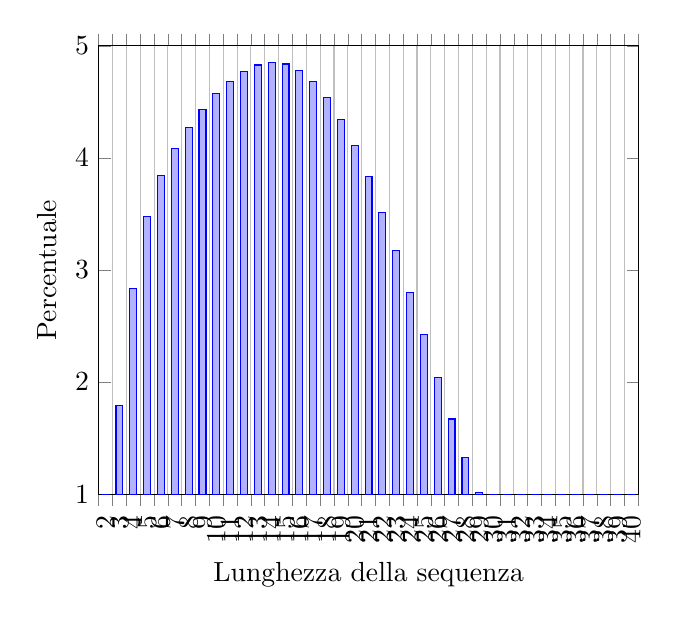
\begin{tikzpicture}
        \begin{axis}[
                ylabel=Percentuale,
                xlabel=Lunghezza della sequenza,
                xmin=2,
                xmax=41,
                ymin=1,
                ymax=5,
                ybar interval=0.5,
                x tick label style={rotate=90},
            ]
            \addplot coordinates {
                    (2,  0.464087)
                    (3,  1.790264)
                    (4,  2.830936)
                    (5,  3.473281)
                    (6,  3.844135)
                    (7,  4.081027)
                    (8,  4.271351)
                    (9,  4.433157)
                    (10, 4.570757)
                    (11, 4.684013)
                    (12, 4.771694)
                    (13, 4.828764)
                    (14, 4.852546)
                    (15, 4.837227)
                    (16, 4.780773)
                    (17, 4.681950)
                    (18, 4.535469)
                    (19, 4.346380)
                    (20, 4.108883)
                    (21, 3.832302)
                    (22, 3.515438)
                    (23, 3.170365)
                    (24, 2.800216)
                    (25, 2.420645)
                    (26, 2.039379)
                    (27, 1.670288)
                    (28, 1.324394)
                    (29, 1.011866)
                    (30, 0.740786)
                    (31, 0.516656)
                    (32, 0.339838)
                    (33, 0.209057)
                    (34, 0.118553)
                    (35, 0.060927)
                    (36, 0.027720)
                    (37, 0.010720)
                    (38, 0.003318)
                    (39, 0.000728)
                    (40, 0.000092)
                    (41, 0)
                };
        \end{axis}
    \end{tikzpicture}
    \caption{Distribuzione statistica delle sequenze}
\end{figure}

\noindent
Possiamo anche analizzare il numero di sequenze corrette e perfette per capire come siano relazionate:

\begin{table}[!h]
    \centering
    \begin{tabular}{@{} c c c c c @{}}
        \toprule
        Sequenze              & Lungezza corrette  & Sequenze perfette  & Percentuale          \\
        \midrule
        \numprint{1000000000} & \numprint{4640873} & \numprint{1406504} & \numprint{30.306884} \\
        \bottomrule
    \end{tabular}
    \caption{Sequenze perfette rispetto alle sequenze corrette, le probabilità sono approssimate a 6 cifre decimali}
\end{table}

\pgfplotsset{width=5cm,compat=1.9}
\begin{figure}[h]
    \centering
    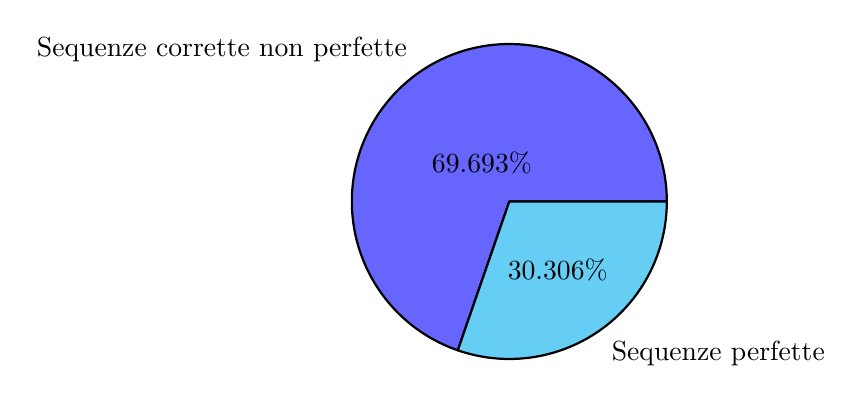
\begin{tikzpicture}
        \pie[radius=2]{ 69.693/Sequenze corrette non perfette, 30.306/Sequenze perfette }
    \end{tikzpicture}
    \caption{Sequenze perfette rispetto alle sequenze corrette}
\end{figure}

\end{document}